%!TEX root = ../main.tex
\section{Simulation}\label{sec:Simulations}
Simulation tools have been a great help, not only in understanding the electromechanical system, and design a controller from it, but also in estimating requirements for the electrical components.
Both Simscape and Plecs Standalone have been used, as they excel at different purposes. 
Simscape is used to test the controller on a system with as much realism as possible to make sure the go-kart functions, whereas Plecs is used to simulate the inverter to determine whether there will be heating issues during operation.

Simscape will be used to simulate how the controller handles certain events:

\begin{itemize}
	\item Actuation of torque pedal.
	\item Speed limitation due to voltage limit.
	\item Release of torque pedal.
	\item Actuation of brake pedal - with and without wheel lock.
\end{itemize}

In all cases, the controller should ensure that the motor produces the requested torque.
The go-kart does not have regenerative braking, so negative torque will be a problem.
The Plecs simulations do not need these details, but the mechanical system still needs a representation of mass of the car, the gear, the wheel and wind resistance. 

\subsection{Mechanical System}\label{sub:Simulations_mec}
The mechanical system consists of a mass of the go-kart with driver, turbulent air resistance, wheels and a gear.

\begin{figure}[H]
	\centering
	\includegraphics[width=15cm]{graphics/simulations_mechanical_full.png}
	\caption{Block diagram of the mechanical system.}
	\label{fig:mechanical_full}
\end{figure}

Figure~\ref{fig:mechanical_full} shows the block diagram of the mechanical part, that the motor will drive.
Starting from the left, the Permanent Magnet Synchronous Motor is the motor and the Ideal Rotational Motion Sensor is used for the Clarke Park transformations. 
The first inertia block contains both the inertia of the motor, which is 0.0052 \si{\kilogram\meter\squared} and the motor-side gear, which can be calculated by equation~\ref{eq:inertia_of_disc}. 
Inertias on the same rod can be added together, so instead of having an inertia for the motor, and one for the motor-side gear, one inertia is enough.
The inertia of the gear depends on its size. 
Assuming, that the gear is a disc, the mass is calculated by:

\begin{equation}
m_{G1} = \rho \pi r^2 \cdot h
\label{eq:mass of disc}
\end{equation}

where $\rho$ is the mass density of iron of $7870 \frac{kg}{m^3}$, $r$ is the radius, and $h$ is the thickness of 7mm.
Radius is defined by the number of teeth of the gear, $G$, and the pitch, which is the distance between two adjacent teeth, which is 12.5mm.
Hence the radius can be calculated by equation~\ref{eq:radius_from_G}
\begin{equation}
	r=\frac{G \cdot d_p}{2 \pi}
	\label{eq:radius_from_G}
\end{equation}

where $d_p$ is the pitch, and $G$ is the number of teeth of the gear. \\

Inertia of a disc depends on mass and radius of the disc according to equation~\ref{eq:inertia_of_disc}.

\begin{equation}
J_G = \frac{mr^2}{2} = \frac{\rho \pi r^2 \cdot h \cdot r^2}{2} = G^4 \frac{\rho \pi \frac{d_p}{2 \pi} \cdot h}{2} \approx 1.36 \cdot 10^{-9} G^4
\label{eq:inertia_of_disc}
\end{equation}

This equation is used to dertermine the inertia of the two gears, the motor-side gear, $G1$, has 12 teeth, and the wheel-side gear, $G2$, has 50 teeth. 
This ratio, $G2/G1$ is put into the block "Gear Box" on figure~\ref{fig:mechanical_full}.
Transferring torque and angular velocity through a gear according to equation~\ref{eq:gear_transfer}.

\begin{equation}
\begin{split}
T_2 = \frac{G_2}{G_1} T_1 \\
\omega_2 = \frac{G_1}{G_2} \omega_1
\end{split}
\label{eq:gear_transfer}
\end{equation}

Since power is the product of torque and speed, which means that power is conserved through the gear.

The mass is set to 150 - 250kg, depending on the driver, and this includes the mass of the car.
This is done to test different situations -- a high mass would have more stable speeds, but also cause more power loss in the inverter, whereas a lower mass would be more prone to wheel spin.\\

Wind resistance represents a larger friction than any other frictions, once the go-kart reach higher speeds.
Wind resistance of a go-kart is primarily turbulent, and can be calculated by equation~\ref{eq:wind_resistance}.

\begin{equation}
\label{eq:wind_resistance}
F=-\frac{1}{2} \rho A c v^2
\end{equation}

where $\rho$ is the density of air, $A$ is the frontal area, $c$ is the drag coefficient and $v$ is the speed. 
The frontal area has been approximated to two rectangles with the combined area of 0.6 \si{\metre\squared}.
The density of air is 1.225\si{\kilogram\per\metre\cubed}, $c$ is approximately 0.8\cite{gokart_constant}.
The constants are multiplied into one constant called $c_{drag}$, as shown in equation~\ref{eq:cdrag}

\begin{equation}
F=c_{drag} v^2 = -0.296 v^2
\label{eq:cdrag}
\end{equation}

These constants are put into the gain block, "Drag coefficient", and multiplied by the square of the speed. 
The result is put into the "force of wind resistance" block, as seen on figure~\ref{fig:mechanical_full}. \\

This system can be simplified, so that all inertia and mass is combined in one block and the gear and wheel can be removed. 
This is done by a set of rules that apply for this mechanical circuit: This gear box reduces the speed, and increases torque, much like a transformer reduces voltage and increases current.
Rotational and translational mechanics are tied together by equation~\ref{eq:rotational_translational}.

\begin{equation}
\begin{split}
T = J \cdot r \\
v = \omega \cdot r
\end{split}
\label{eq:rotational_translational}
\end{equation}

To turn the mass of the vehicle, m, into an inertia, assume that the entire mass is mounted on the surface of the driving wheels. 
This means, the inertia can be considered a shell with mass m, and radius r, in which case, inertia can be calculated as:

\begin{equation}
J=mr^2
\end{equation}

Since the mass is now transformed into an inertia, it can be added to the inertia $J_{G2}$.\\

Same rules apply for a gear as for a transformer when reflecting a load from one side to the other.
This means, that a torque source driving an inertia through a gear, is experiencing an inertial load calculated by equation~\ref{eq:inertia_reflect}.

\begin{equation}
\label{eq:inertia_reflect}
J_{ref} = \frac{G1^2}{G2^2} J
\end{equation}

This inertia is then added to the inertia of the motor and $\mathrm{J_{G1}}$:

\begin{equation}
J = (mr^2+J_{G2}) \cdot \big(\tfrac{G1}{G2}\big)^2 + J_{G1}+J_M
\end{equation}
%
In equation~\ref{eq:cdrag}, speed can be replaced with angular velocity and a gear ratio, and force can be replaced by torque and the gear ratio, according to equation~\ref{eq:rotational_translational}. So the equation becomes this:

\begin{equation}
\frac{T G2}{r G1} = c_{drag} \cdot \big(\omega r \tfrac{G1}{G2}\big)^2
\end{equation}

Isolating $T$results in:

\begin{equation}
T= c_{drag} \Big(\frac{G1 r}{G2}\Big)^3 \omega^2 \approx -11.1\cdot 10^{-6} \omega^2
\end{equation}

The mechanical diagram is reduced to figure ~\ref{fig:reduced_mechanical_system}

\begin{figure}[H]
	\begin{center}
	\includegraphics[width=12cm]{graphics/simulations_mechanical_simplified.png}
	\caption{Block diagram of the reduced mechanical system.}
	\label{fig:reduced_mechanical_system}
	\end{center}
\end{figure}

In the Simscape model, the tyre is modelled by a friction block in series with the rotor, and the brake is modelled in a subsystem, as seen on figure~\ref{fig:simulations_mechanical_simscape}.

\begin{figure}[H]
	\begin{center}
		\includegraphics[width = 12cm]{graphics/simulations_mechanical_simscape.png}
		\caption{Block diagram for the mechanical system used in Simscape.}
		\label{fig:simulations_mechanical_simscape}
	\end{center}
\end{figure}

The tyre block consists of static and dynamic friction.
Tyre slip is a comprehensive area of study, so the rotational friction block isn't necessarily accurate. 
However, it does enable sudden changes in motor speed and load, similar to spinning and locking the wheels.
The tyre block consists of static, dynamic and viscous friction. The static and dynamic frictions are are calculated by equation~\ref{eq:static_dynamic_friction}

\begin{equation}
F_f = F_N \cdot c_f \cdot dm
\label{eq:static_dynamic_friction}
\end{equation}

where 

\begin{equation}
F_N = mg \cdot dm
\end{equation}

and $c_f$ is either the static or dynamic friction, depending on if the wheels are slipping. 
The constant, dm is the distribution of mass so that $dm=0$ means the entire mass of the go-kart is on the front wheels, and $dm=1$ means the whole weight distribution is on the driving wheels.
The viscous friction is zero.
The static friction coefficient is 1, the dynamic friction is 0.7, and the mass distribution is 0.6.

The brake subsystem is a PI controlled ideal torque source, which will attempt to bring the go-kart to a halt when the brake is pressed.
Without a PI controller, there is a strong possibility that the brake would suddenly make the motor go backwards instead of stopping.\\
Lastly the inertia is split into two inertia blocks, one containing motor and gear inertia on the left of the tyre, and the inertia due to the mass of the car on the right.
The brake on the go-kart is mounted on the rear axle, which means the torque it produces must be scaled down to represent the torque seen on the motor rod.

\subsection{Motor Model}\label{sub:motor_model_simscape}
Both Simscape and Plecs have built in models of PMAC motors.
They have the four basic parameters: Number of pole pairs, flux linkage of the magnet, inductance and armature resistance. 
The parameters used for simulations are listed in table~\ref{tab:motor_parameters_in_simulations}.

\begin{table}[h]
	\centering
	\begin{tabular}{| S | S |}
		\hline
		\rowcolor[HTML]{C0C0C0}{Parameters} &  {Value} \\
		\hline
		{Flux linkage} & {$0.0183$} \\
		\hline
		{$L_d$, $L_q$, $L_0$}& {$4\cdot10^{-5}$}\\
		\hline
		{Rs} & {6.5e-3}\\
		\hline
		{Pole pairs} & {4}\\
		\hline
	\end{tabular}
	\caption{Parameters used in simulations.}
	\label{tab:motor_parameters_in_simulations}
\end{table}

One thing to note is that the flux linkage is divided by the number of pole pairs.
The reason for this is likely a matter of definitions, and the relation has been deduced using simulations. 
Armature resistance and inductances are per-phase, and the values used are found in section~\ref{sub:1117_param}.

\subsection{Electrical Network and Control}\label{sub:sim_electrical}
The electrical network along with the discrete controller and modulation blocks are shown in figure~\ref{fig:simulations_electrical}.
This section will explore the performance of the controllers.

\begin{figure}[h]
	\begin{center}
	\includegraphics[width=16cm]{graphics/simulations_electrical.png}
	\caption{The Simulink electrical network and modulation.}
	\label{fig:simulations_electrical}
	\end{center}
\end{figure}

The motor block has an external connection to neutral, which the real motor doesn't have. 
This neutral seems to need a DC path to ground, and so does the controlled voltage sources. 
Since the external ground cannot be connected to the internal star point of the motor, the connection is made with a very large resistor of 1\si{\giga\ohm}. 
The lighter blue wire going into the "\texttildelow" port of the PMSM block is a three phase electrical cable, which is used throughout the SimPowerSystem sublibrary, and the Splitter collects three wires into a cable. \\

Current is sensed on wires A and B, and used to calculate $I_C$ in the Zybo block.

The angular position is measured with an ideal position sensor, and then sent to the encoder block.
Here, the finite precision of the encoder is simulated by equation~\ref{eq:Encoder_block_function}

\begin{equation}
\label{eq:Encoder_block_function}
output = \left\lfloor \Bigg( \frac{\phi \cdot 256}{2 \pi} + 0.5 \Bigg) \% 256\right\rfloor
\end{equation}

where \% is the modulo function. 
The purpose of that is to wrap the output to a value between 0 and 255, which can be used for look-up tables. 
The round down function rounds a number, effectively quantizing the output. 
The reason for using round down rather than just round is to ensure, that the number ranges from 0 to 255. 
The rounding error is minimized by adding 0.5. 
It has been attempted to use the quantizer block, but that causes stiffness to the point where the simulation almost stalls. 
The output is sent to the Zybo block, which will be explained in section~\ref{sub:sim_zybo}.\\

The Zybo subdiagram generates duty cycles for each phase ranging from -1 to 1. 
This value is then multiplied with 26.4\si{\volt} to represent half the battery voltage, and then saturated to ensure, that the ideal voltage sources do not provide more voltage than possible.
\subsubsection{Zybo block}\label{sub:sim_zybo}
The Zybo block consists of three other subsystems, corresponding with some of the blocks on the actual Zybo; Clarke Park, Discrete controller and PWM generation.
This can be seen on figure~\ref{fig:simulations_zybo}.

\begin{figure}[H]
	\begin{center}
		\includegraphics[width = 12cm]{graphics/simulations_zybo}
		\caption{Block diagram describing the Zybo part of the system.}
		\label{fig:simulations_zybo}
	\end{center}
\end{figure}

The Clarke Park transform and PWM generation blocks are running in variable time steps, and the discrete controller runs with a fixed step of 0.1 \si{\milli\second}.
The signal builder block is used to shape the torque requested by the pedal.
This torque is converted into the current used in the controller by multiplying with $\tfrac{3}{2 K_t}$.
The Clarke Park block converts $I_{AB}$ to $I_{dq}$. 
Due to the limitations of the encoder, the system only measures 64 different electrical angles.

The block diagram of the discrete controller is shown on figure~\ref{fig:sim_controller_diagram}.

\begin{figure}[H]
	\centering
	\includegraphics[width = 16cm]{graphics/sim_controller_diagram}
	\caption{Block diagram of discrete PI controller.}
	\label{fig:sim_controller_diagram}
\end{figure}

The two independent current controllers are drawn in blue boxes. 
The feedback comes from the $I_{dq}$ port on the left.
The constants, $K_p$ and $K_i$, are calculated in section~\ref{sec:controller_design}, and divided by half the battery voltage.
This is done, because the controllers designed in section~\ref{sec:controller_design} produce a voltage, whereas the simulink controller produces a percentage of half the battery voltage, i.e. between -1 and 1.
Similarly the implemented PWM block in section~\ref{sub:Architecture} takes integers in the range from 0 to 1000, so the controller constants need to be scaled accordingly\\
The integrator block uses trapezoidal integration, and the output is limited to $\pm \tfrac{2}{\sqrt{(3)}}$.
This is to ensure, that the integrator does not wind up.
The saturation block to the left of the q current controller on figure~\ref{fig:sim_controller_diagram} limits the input to between 0 and a maximum current.
The PI controllers produce duty cycle values in the range of $\mathrm{\pm \tfrac{2}{\sqrt{(3)}}}$, although it is possible to exceed this range at this point in the diagram.\\

It is necessary to ensure, that the controller does not produce values outside the range that can be generated using PWM. 
The obvious solution is to put a saturation block after each of the controllers, but a large value value from both controllers will still cause saturations.
In order to limit both controller outputs without disturbing the controllers, both output values is reduced by the same factor. 
The magnitude of the dq-duty cycle vector must not exceed $\tfrac{2}{\sqrt{3}}$, when using third harmonic injection. 
For this reason, the magnitude of the two controller outputs is calculated in the red box. 
If the magnitude is larger than $\tfrac{2}{\sqrt{3}}$, the Parallel scale down subsystem is processed. 

For comparison, the d and q axis duty cycles have been simulated and are shown on figure~\ref{fig:parallel_scale_down_graphs}: 

\begin{figure}[H]
	\centering
	\begin{subfigure}[t]{.49\linewidth}
		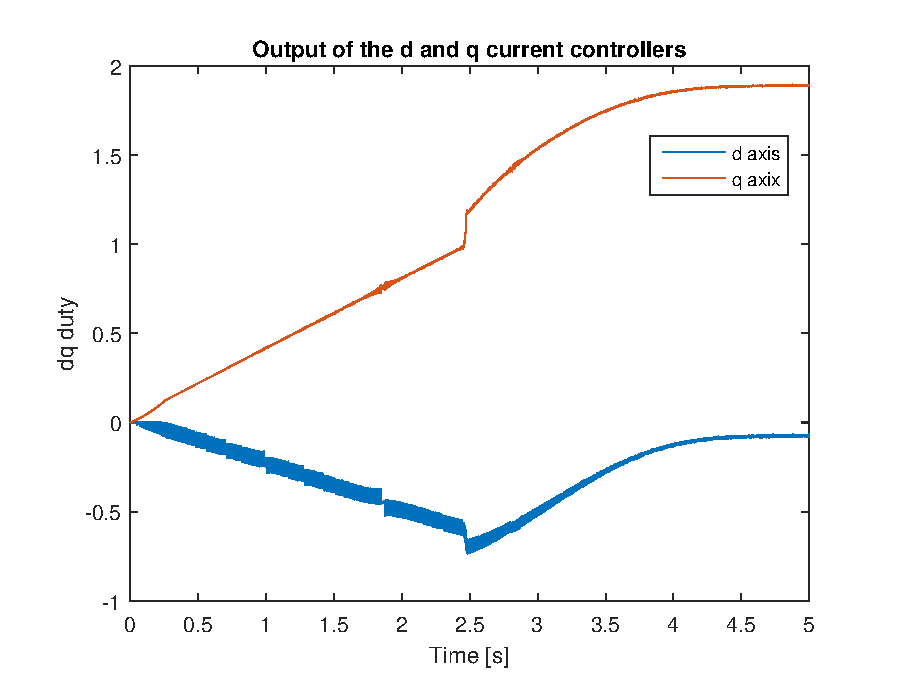
\includegraphics[width=\textwidth]{graphics/before_saturation}
		\caption{Before parallel scale down.}
		\label{fig:before_saturation}
	\end{subfigure}
	\begin{subfigure}[t]{.49\linewidth}
		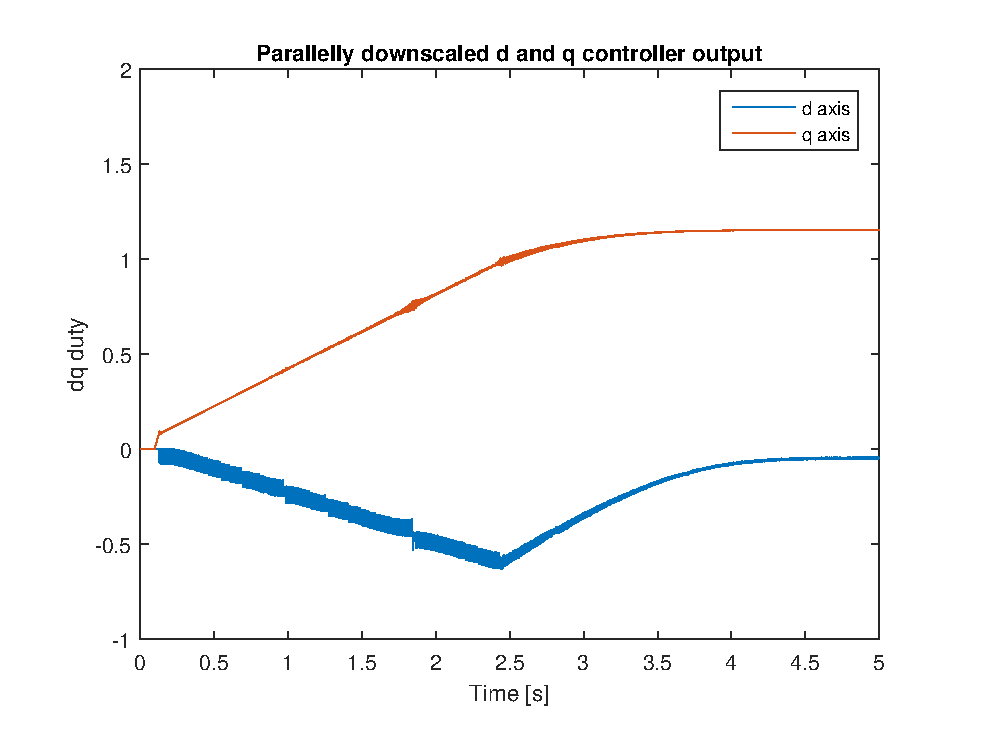
\includegraphics[width=\textwidth]{graphics/after_saturation}
		\caption{After parallel scale down.}
		\label{fig:after_saturation}
	\end{subfigure}
	\caption{dq duty cycle values before and after parallel scale down.}
	\label{fig:parallel_scale_down_graphs}
\end{figure}

The graphs are simulated with a car mass of 200\si{\kilogram}, and settling time of 0.01s.
At 2.5s, the magnitude of the dq-vectors exceeds $\tfrac{2}{\sqrt{(3)}}$, at which point both the d and q output is scaled down. 
On figure~\ref{fig:after_saturation}, this transition is almost invisible along the q-curve. 
As the torque produced by the motor is reduced due to saturation of the supply, the need for a large negative d-duty is reduced, as both d and q current is reduced.

\begin{figure}[H]
	\centering
	\includegraphics[width = 14cm]{graphics/sim_PWM_generation}
	\caption{Block diagram of the PWM generator.}
	\label{fig:sim_PWM_generation}
\end{figure}

The majority of this block diagram calculates the inverse Clarke Park transformation, and in the upper right corner, the third harmonic injection is calculated using the knowledge given in \cite{third_harmonic_injection}. \\


The issue is that, when using field oriented control, the stator voltage does not remain at a constant angle relative to the rotor angle.
That means, that calculating the third harmonic isn't as simple as multiplying the rotor position with three. 
Doing this will result in the the third harmonic being out of phase with the three sinusoidal voltage waveforms as speed increases.
This will result in higher peak voltages at certain speeds.
Instead, the third harmonic needs to be calculated from the dq output from the controller. \\

Equation (9) in the paper\cite{third_harmonic_injection} defines the three phase voltage of a balances system without third harmonic injection:

\begin{equation}
\left[ \begin{array}{c}
V_A \\ V_B \\V_C
\end{array} \right]
=
\left[ \begin{array}{c}
V \sin(\Theta) \\
V \sin(\Theta - 120 \si{\degree}) \\
V \sin(\Theta + 120 \si{\degree})
\end{array} \right]
\label{eq:equation_9}
\end{equation}

where $\mathrm{\Theta}$ is the instantaneous phase, and V is the instantaneous magnitude, calculated as:

\begin{equation}
V = \sqrt{V_q ^2 + V_d ^2}
\label{eq:v_from_vdq}
\end{equation}

Note that equation~\ref{eq:v_from_vdq} is not equal to equation 10 in the paper\cite{third_harmonic_injection}, because this dividing with 1.5 is done in the Clarke Park transform block. 

From equation~\ref{eq:equation_9}, we know that:

\begin{equation}
\Theta = \sin^{-1} \Big(\frac{V_A}{V}\Big)
\label{eq:equation_11}
\end{equation}

The third harmonic sinusoidal is given in equation (12) of the paper\cite{third_harmonic_injection}, and shown in equation~\ref{eq:v_th}

\begin{equation}
V_{th} = \frac{1}{6} \sin(3 \Theta) = \frac{1}{6} \sin\Bigg(3 \sin^{-1} \Big(\frac{V_A}{V}\Big)\Bigg)
\label{eq:v_th} 
\end{equation}

This third harmonic sinusoidal is added to each of the phases, as shown in equation~\ref{eq:equations_14}

\begin{equation}
\begin{bmatrix}
V_{Ath} \\
V_{Bth} \\
V_{Cth}
\end{bmatrix}
=
\begin{bmatrix}
V_A + V_{th} \\
V_B + V_{th} \\
V_C + V_{th}
\end{bmatrix}
\label{eq:equations_14}
\end{equation}

This allows the controller to go beyond the full range of the voltage without saturating. \\

The reason this third harmonic injection is only enabled when the magnitude is larger than zero is to avoid dividing by a negative number in equation~\ref{eq:equation_11}.

\subsection{Simulation Results}\label{sub:simulink_results}
The simulation will be run with both PI and IP controllers, with values described in sections~\ref{sub:full_order_controller_values} and~\ref{sub:reduced_order_controller_values}. \\

\subsubsection{PI controller}\label{sub:PI05}
Throughout this section the PI controller developed in section \ref{sec:controller_design} for a full order system will be tested.
At first, a simulation will be run where the throttle is pressed fully from 0.12s to 5s, and then released.
This input is similar to the one used in section~\ref{sec:controller_design}.
The mass is 200kg.
The resultant current along the d and q axes have been plotted in figure~\ref{fig:Sim_results_pi_Idq}.

\todo[inline]{Input signal needed}
\begin{figure}[H]
	\centering
	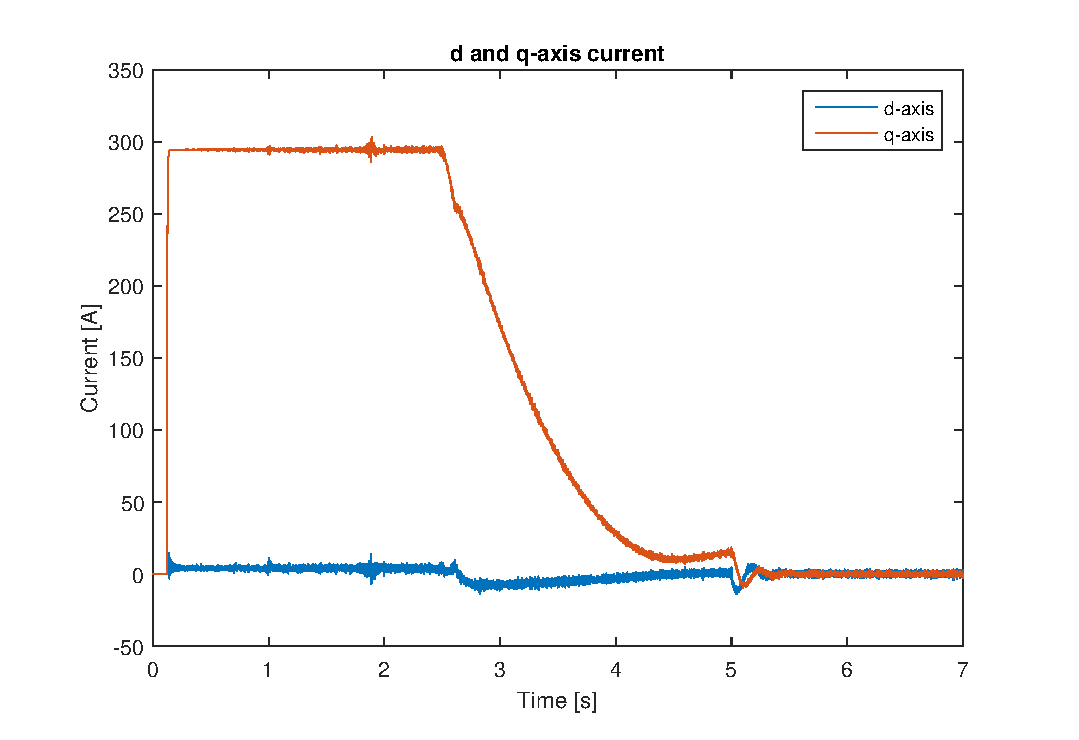
\includegraphics[width=0.7\linewidth]{graphics/Sim_results_pi_Idq}
	\caption{d and q current simulated with a positive and negative step.}
	\label{fig:Sim_results_pi_Idq}
\end{figure}

Much like on figure~\ref{fig:Output_Full}, the current steps up nicely with almost no overshoot. 
There is also a small steady state error of about 2 \%, as was the case in section \ref{sec:controller_design}.
There is a small current noise on $I_q$ and especially $I_d$, which is caused by the quantization of the encoder.
Using a higher frequency for the discrete controller reduce this ripple. 
For these simulations, 10\si{\kilo\hertz} has been used
lower frequencies can be used with acceptably low noise, up to 0.5\si{\kilo \hertz}.
The extra noise on both the d and q current at 1.8\si{\second} is imaging error, caused by the quantization of the encoder and the frequency of the controller.
For controller frequency, the error happens when the motor is running at 2250 RPM.
Lower frequencies mean, that the error happens at lower motor speeds. \\
The d-axis current is kept very close to zero, at least until 2.6 seconds, when the voltage starts saturating. 
A small error (of up to -20 A) is not a big issue, as this is likely to occur anyway if the position encoder is not perfectly aligned.\\
When saturation occurs, the current drops off almost exponentially. 
At 5 seconds, when the throttle is released, both the d and q current ripples a bit. 
This is due to the way saturation is handled, but the ripple is not a major ground for concern.

The voltage waveforms must not be saturated, and should remain sinusoidal with third harmonic injection.
This is shown on figure~\ref{fig:Sim_results_pi_phase_voltage}

\begin{figure}[H]
	\centering
	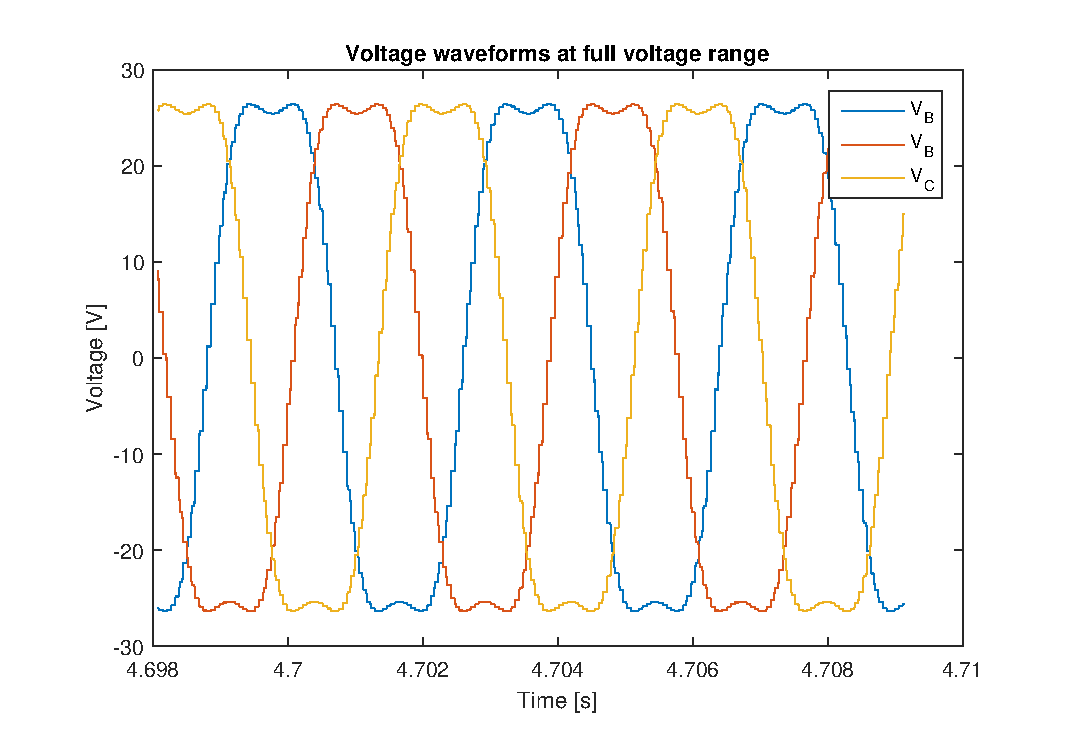
\includegraphics[width = 0.7\linewidth]{graphics/Sim_results_pi_phase_voltage}
	\caption{Voltage waveforms measured when the motor is running at 4000 RPM.}
	\label{fig:Sim_results_pi_phase_voltage}
\end{figure}

The reason for stepping voltage instead of a smooth curve is the limited resolution of the encoder. 
This is not an issue, because these steps will induce a high frequency noise, that the inductance of the motor will filter out.
Figure~\ref{fig:Sim_results_pi_phase_voltage} shows that the voltage waveforms span the whole range, even at speeds where the controller output is outside the $\pm1.15$.
This works independently from the controller, and will work both for the PI and IP controller. \\

When the throttle is released after 5s, the power should ideally not become negative, as the inverter is not designed to handle regenerative braking.
This means, that it is not known what happens if the motor tries to push power back to the battery.
Figure~\ref{fig:Sim_results_pi_phase_power} shows a short power undershoot occurring when the controller input goes from full to zero.

\begin{figure}[H]
	\begin{subfigure}[b]{.49\linewidth}
		\centering
		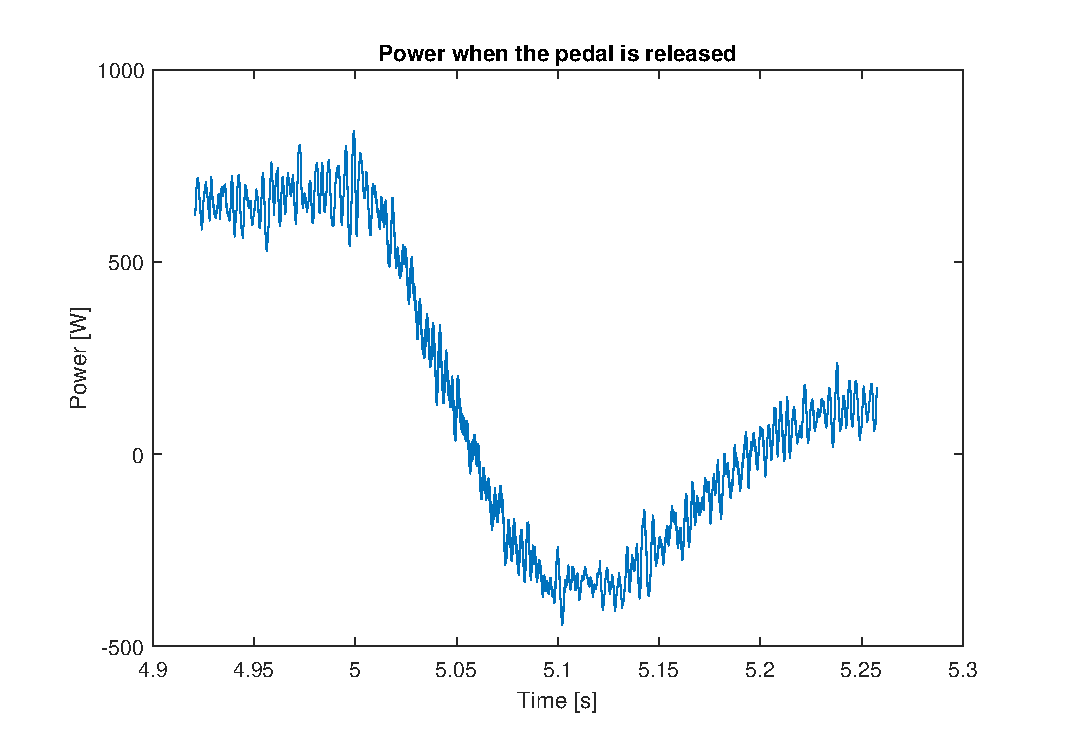
\includegraphics[width = \linewidth]{graphics/Sim_results_pi_phase_power}
		\caption{Power undershoot when throttle is released.}
		\label{fig:Sim_results_pi_phase_power}
	\end{subfigure}
	\begin{subfigure}[b]{.49\linewidth}
		\centering
		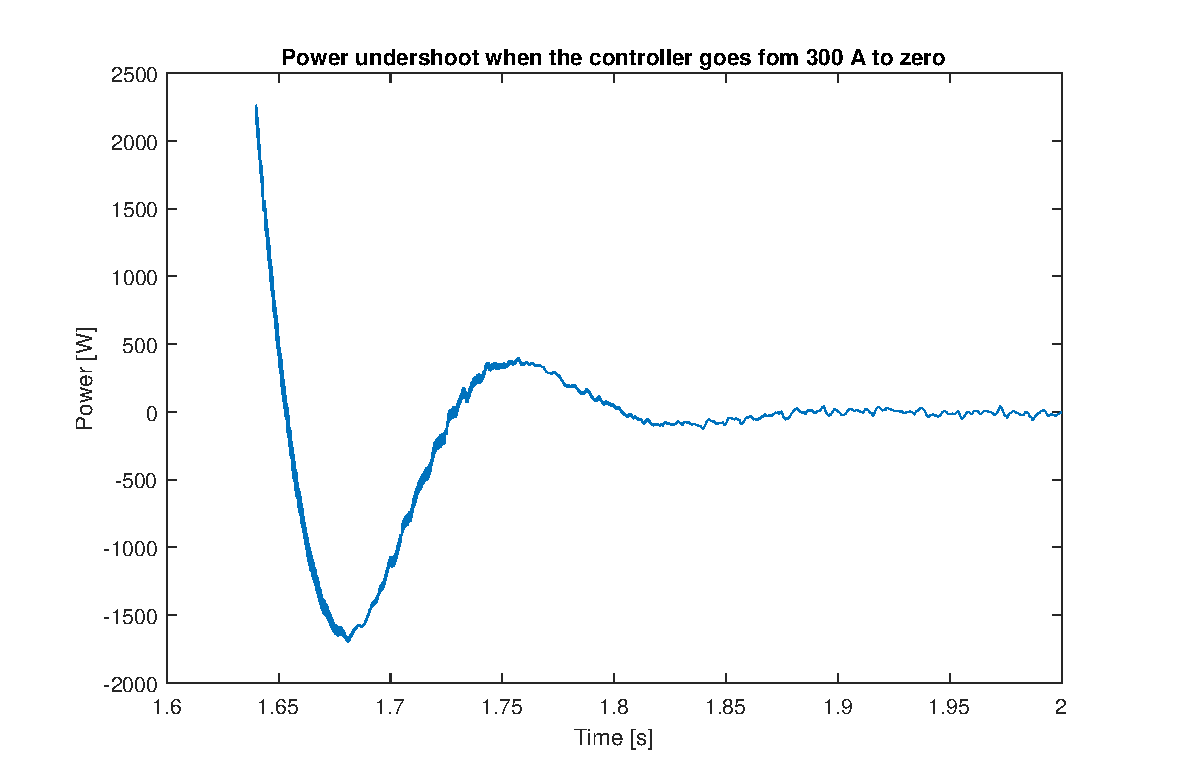
\includegraphics[width = \linewidth]{graphics/Sim_results_pi05_large_power_undershoot}
		\caption{Power undershoot crosses zero 33 ms after the throttle is released.}
		\label{fig:Sim_results_pi05_large_power_undershoot}
	\end{subfigure}
	\caption{Undershoot when releasing torque pedal.}
\end{figure}

The power peaks at -400\si{\watt} for a short time.
Integrating the power from 5.06 to 5.5s gives an energy of -25\si{\joule}.
This is not likely to cause problems, as this energy easily could be lost in the inverter.
The issue is larger when releasing the throttle while the go-kart is accelerating. 
This is shown on figure~\ref{fig:Sim_results_pi05_large_power_undershoot}.

Integrating this undershoot yields -62\si{\joule}. 
This is not a major concern, however it causes a ripple in the speed, that might be felt. \\

\subsubsection{IP controller}\label{sub:IP05}
Throughout this section the IP controller developed in section \ref{sec:controller_design} for the reduced order system is tested.
In order to do that, the wire going into the Kp gain block must be connected with the feedback wire, instead of the output of the summation block

\begin{figure}[H]
	\centering
	\includegraphics[width = 0.75\linewidth]{graphics/ip_controller_in_full_system}
	\caption{Input to $\mathrm{K_p}$ gain blocks are connected to the $\mathrm{I_{dq}}$ feedback wire instead of the output of the summation block.}
\end{figure}

The parameters are divided by half the battery voltage, and shown in equation~\ref{eq:IP_controller_constants}.

\begin{equation}
K_P = -2.65e-5 \\%1515151515156e-05
K_I = 1.23e-2 %0.012272727272727
\label{eq:IP_controller_constants}
\end{equation}

Figure~\ref{fig:Sim_results_ip_Idq} shows the d and q-axis current as the controller is given a positive and a negative step.
\todo[inline]{refer to input figure}

\begin{figure}[H]
	\begin{subfigure}[t]{.49\linewidth}
		\centering
		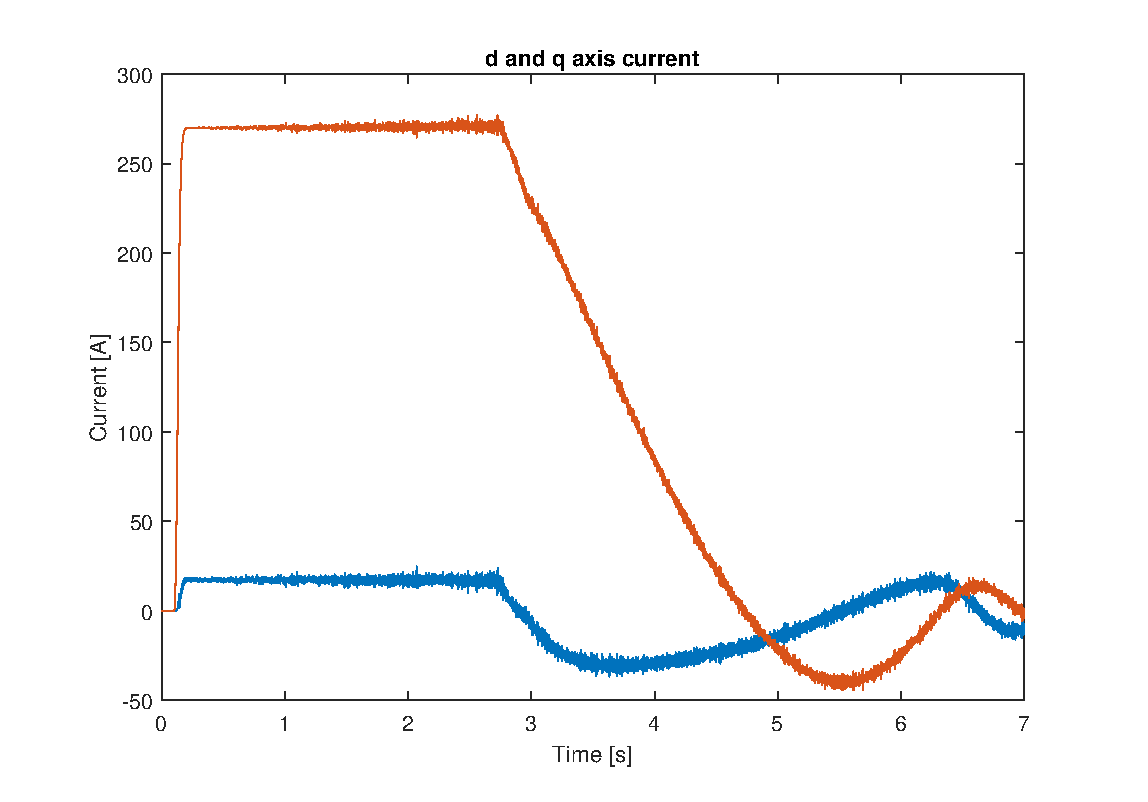
\includegraphics[width = \linewidth]{graphics/Sim_results_ip_Idq}
		\caption{d and q axis current with a positive and negative step with the IP controller.}
		\label{fig:Sim_results_ip_Idq}
	\end{subfigure}
	\begin{subfigure}[t]{.49\linewidth}
		\centering
		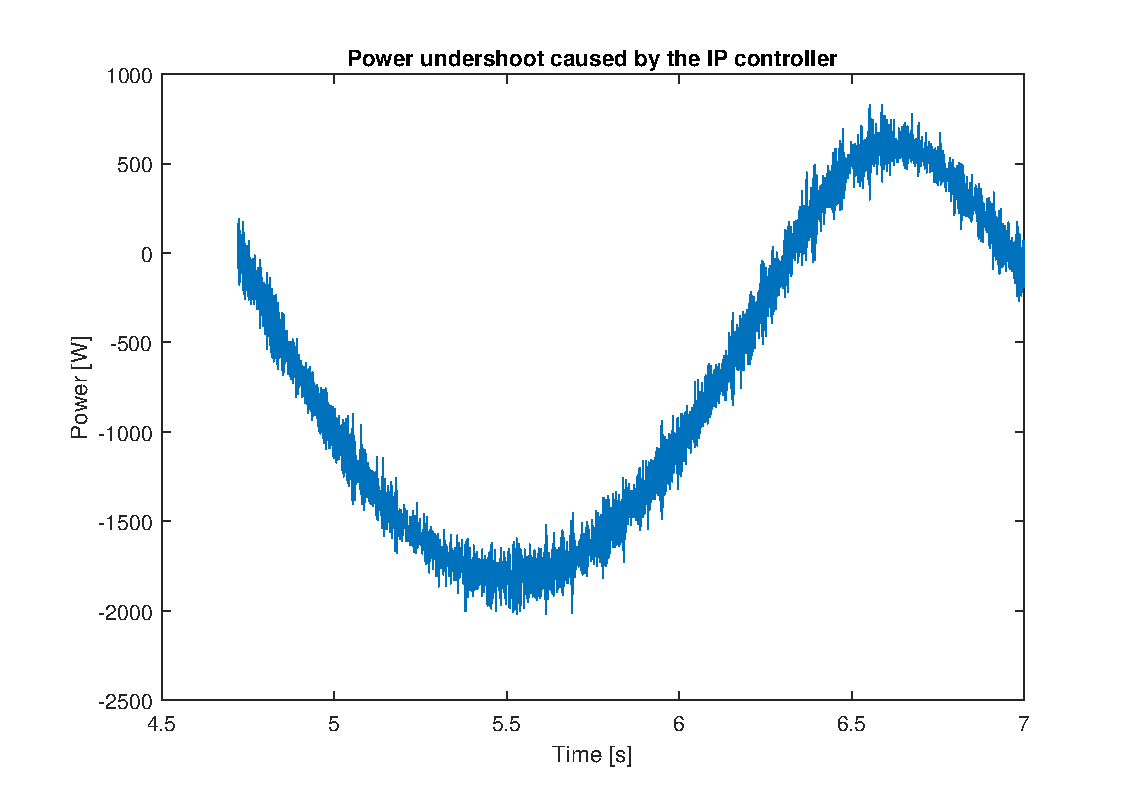
\includegraphics[width = \linewidth]{graphics/Sim_results_ip_power}
		\caption{Negative power caused by oscillation.}
		\label{fig:Sim_results_ip_power}
	\end{subfigure}
	\caption{Characteristics of IP controller.}
\end{figure}

By comparison to the PI controller, the IP controller does significantly worse.
The steady state error of the q-controller is 10\%, while the d-controller has a steady state error of $d16\si{\ampere}$.
What's even worse is, that the q-axis current goes below zero before the throttle is released after $5\si{\second}$.
That means, that when driving the go-kart at full throttle, the speed of the go-kart will start oscillating quite notably.
At 5 seconds, the throttle is released, at which point the current should be zero. 
The current is already at $-22\si{\ampere}$ at this point, and the negative step does not seem to alter the oscillation in any way.
The negative torque causes a negative power, as shown in figure~\ref{fig:Sim_results_ip_power}

A power of this magnitude is likely to cause serious damage to the inverter, if it's lost in the inverter, and not used to charge the battery.
The total energy being delivered back in the timespan shown on figure~\ref{fig:Sim_results_ip_power} to the inverter is 1614J.\\

\subsubsection{PI Controller with Faster Settling Time}\label{sub:PI01}

Since neither of the two controller designs work optimally, the PI controller will be redesigned with a settling time of $\mathrm{10 \si{\milli \second}}$.
The controller is designed for a load of $\mathrm{200 \si{\kilogram}}$.
The control parameters in equation~\ref{eq:10ms_settling_time_param} are divided by half the battery voltage

\begin{equation}
\begin{split}
K_P &= 1.64 \\%1.637719093817946
K_I &= 2.6 \cdot 10^{-3} %0.002604159942864
\end{split}
\label{eq:10ms_settling_time_param}
\end{equation}

The reason for not using the settling time of 1\si{\milli\second} is, that it provides a large overshoot, which was also evident in this more elaborate simulator.
Introducing a rate limiter block in the Discrete controller subsystem between the q setpoint port and the saturation block will reduce the overshoot to less than 1\%.
This block is displayed on figure~\ref{eq:IP_controller_constants}.
The rising and falling rates are set to $\mathrm{10 \si{\kilo \ampere \per \second}}$ and $\mathrm{-10 \si{\kilo \ampere \per \second}}$.
This is fast enough, that a driver would not notice.

Figure~\ref{fig:Sim_results_pi01_Idq} shows the positive and negative current step.

The faster $\mathrm{I_{q}}$-controller is much more precise.
The rate limiter ensures, that the overshoot is less than 1 percent.
The steady state error negligible.
However, the $\mathrm{I_{d}}$-controller is more noisy, but still close to zero.
There is a small current undershoot when the pedal is released of only -3\si{\ampere}. The power caused by this is shown on figure~\ref{fig:Sim_results_pi01_power}

\begin{figure}[H]
	\begin{subfigure}[t]{.49\linewidth}
		\centering
		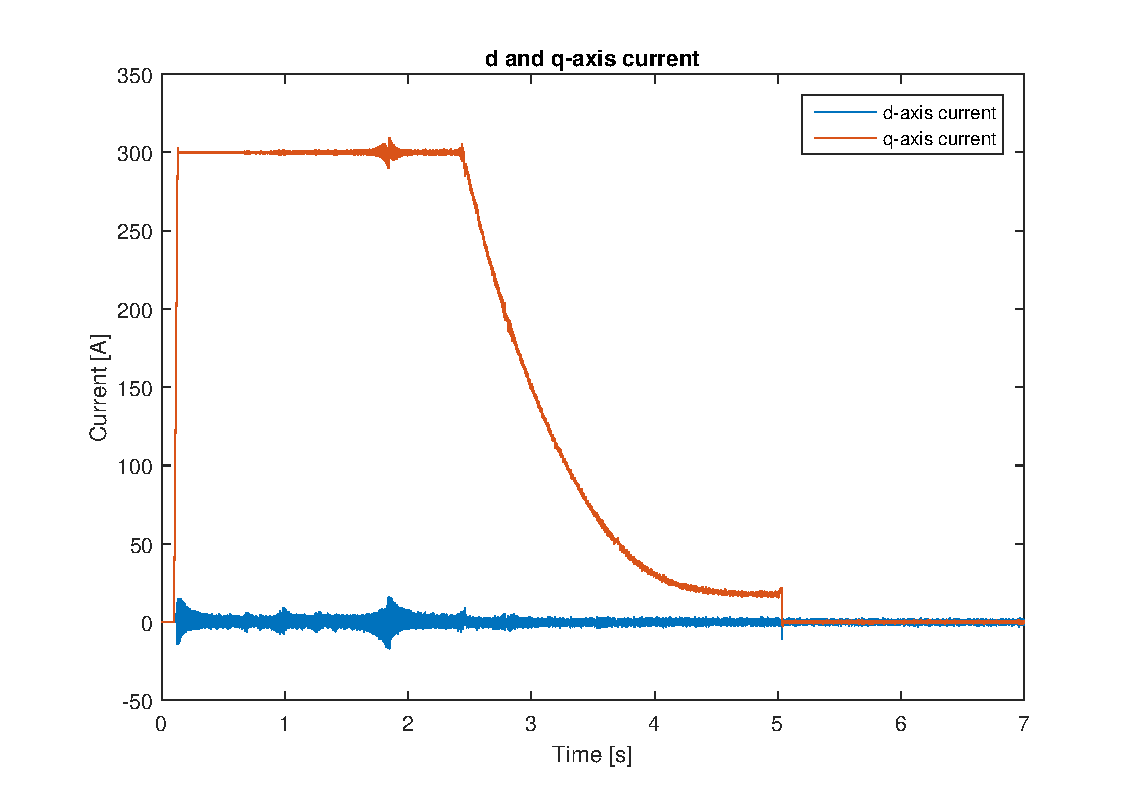
\includegraphics[width = \linewidth]{graphics/Sim_results_pi01_Idq}
		\caption{d and q axis current is a lot more precise than on figure~\ref{fig:Sim_results_pi_Idq}.}
		\label{fig:Sim_results_pi01_Idq}
	\end{subfigure}
	\begin{subfigure}[t]{.49\linewidth}
		\centering
		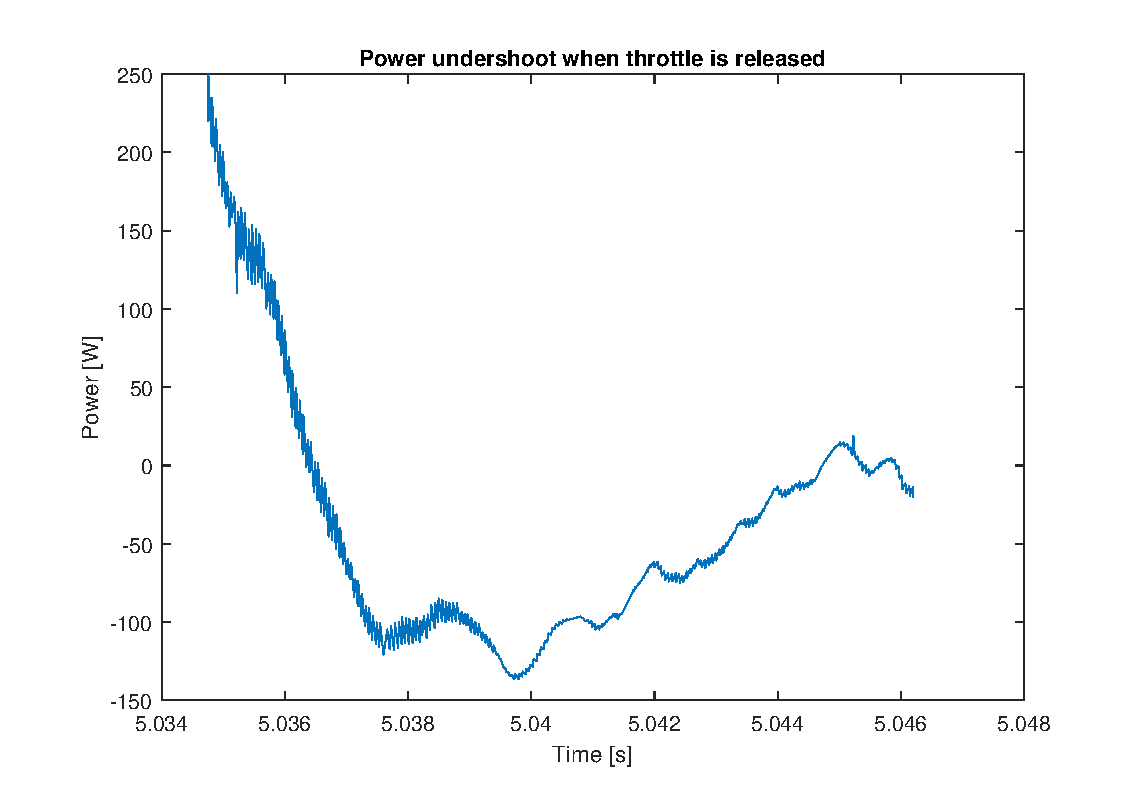
\includegraphics[width = \linewidth]{graphics/Sim_results_pi01_power}
		\caption{A short and small current undershoot of only 0.6 \si{\joule}}
		\label{fig:Sim_results_pi01_power}
	\end{subfigure}
	\caption{Characteristics of IP controller.}
\end{figure}

The power undershoot is significantly smaller, and lasts for a shorter time, meaning that the energy returned to the inverter is reduced from 25 \si{\joule} to just 600 \si{\milli \joule}.

\subsubsection{Conclusion of Controller Comparison}\label{sub:simulink_conclusion}

The control parameters have been tested on a highly detailed physics simulator, with the conclusion, that neither the PI controller based on the mechanical system, nor the IP controller based on a reduced order system works satisfactorily.
A faster controller was calculated with tremendous results.

\begin{table}[H]
	\centering
	\begin{tabular}{|c || c | c | c |}
		\hline
\rowcolor[HTML]{C0C0C0}		{Event} & {PI controller} & {IP controller} & Fast {PI controller} \\
		\hline
		{Torque step} & {Handles well} & {Slow, steady state error} & {Excellent}\\
		\hline
		{Speed limit} & {Great. Same for all} & {Great. Same for all} & {Great. Same for all} \\
		\hline
		{Torque release} & {Small power returned}& {Oscillation}& {Great response}  \\
		\hline
	\end{tabular}
	\caption{Table comparing the abilities of the three tested controllers.}
	\label{tab:simulink_conclusion}
\end{table}

\todo[inline]{make gray}

Both the PI controllers could work, but the faster response gives very precise current control.
The IP controller was designed in section~\ref{sec:controller_design} based on a reduced order system without any mechanical part. 
Evidently, the motor along with the mass of the go-kart has a slow pole, that the IP controller does not handle.
The IP controller adds a pole to the systems, which makes the fast pole on figure~\ref{fig:PZmap_reduced_v2} complex conjugate poles that can oscillate.
This oscillation proves to be too much when adding the slow poles of the mechanical system.
As it has shown, this controller is not able to account for the mechanical system as a disturbance, which is unsurprising really giving the scope of the mechanics involved.
It was found that the PI controller designed for the lowest settling time showed the best performance.
Further tuning of the control variables could potentially yield better results.
\subsection{Plecs model}\label{sub:sim_plecs_electrical}
The reason for using Plecs is that it handles semiconductors as ideal switches.
This greatly reduces the time required to simulate switch mode voltages.
As both the high side and low side MOSFETs of each phase switch simultaneously, each PWM period of simulation contains up to six switching events. 
At 20 kHz, this means, the whole circuit needs to be solved 120.000 times per second, so using plecs is still not fast.
The main use of this model is the simulation of heat dissipation throughout the circuit.

As previously mentioned, the Plecs model differs vastly from the Simulink model in the electrical network, as it more closely resembles the real analog circuit. 
It is shown on figure~\ref{fig:plecs_electrical}.
\todo[inline]{make vertical!}
\begin{figure}[H]
	\begin{center}
		\includegraphics[width = \linewidth]{graphics/Plecs_electrical}
		\caption{Block diagram for the svm plecs simlations.}
		\label{fig:plecs_electrical}
	\end{center}
\end{figure}

The simulation utilizes the fast PI controller from page~\pageref{sub:PI01}. 
It simulates the switching inverter utilizing ideal switches as opposed to more realistic MOSFETs with limited current rate of change. 
Because of the ideal switching, it is not necessary to include antiparallel diodes, nor deadtime.

Figure~\ref{fig:plecs_electrical} shows the three phase inverter.
The blue rectangle around each mosfet is a heatsink, that absorbs all the power loss within it.
These are used to emulate the case of the transistors. 
Each of these have a heat capacity of 0.01 \si{\kelvin \per \joule } \\ 
Each transistor represent one pair of transistors, where the on-resistance is zero.
The transistors have the same thermal model, with look-up tables for switch-on and switch-off energies based on equation~\ref{eq:P_sw}.
The energy lost per switch is calculated by equation~\ref{eq:plecs_switching_losses}.

\begin{equation}
E_{on} = \frac{1}{2} V_{DS} \cdot |I_D| \cdot t_{c,on} \\
E_{off} = \frac{1}{2} V_{DS} \cdot |I_D| \cdot  t_{c,off}
\label{eq:plecs_switching_losses} 
\end{equation}

Because a negative current would cause the same loss, as a positive current, the absolute is taken of the drain current.
All losses are calculated for two MOSFETs in parallel, conducting the combined current.

Conduction loss is dependent on the temperature of the mosfet. 
This however, does not change the on-resistance in the circuit, this is not possible to do in Plecs.
It should be noted, that the heatsink-box includes all losses inside, meaning it includes both the loss specified in the thermal model, but also the loss due to a non-zero on-resistance. 
This is part of the reason, the on-resistance has been set to zero, the other part being faster simulation. \\

All heatsink boxes are connected through a thermal resistor (the blue ones) to a shunt thermal capacitor (CthG).
The thermal resistance of 0.145 \si{\joule \per \kelvin} represents the case-to-sink thermal resistance as read from the datasheet.
The datasheet value was divided by two, because there are two TO-247 houses conducting the heat.
CthG along with Heatsink Thermal Resistance models the 30x30 heatsink used to mount the inverter. 
CthG has a thermal capacity of 2100 \si{\kelvin \per \joule}, which is based on its size and the thermal capacity of aluminium, according to~\ref{eq:thermal_capacity}.

%\begin{equation}
%C_{th} = v \cdot \rho_m C_{p}
%\label{eq:thermal_capacity}
%\end{equation}

%where $C_{p}$ is the specific heat capacity of aluminium, which is 910 \si{\joule\per\kilogram\kelvin}, and $\rho_m$ is the mass density of aluminium.
%For a heatsink of 30x30x1\si{\centi\metre}, the heat capacity is 2180 \si{\kelvin \per \joule}.

The battery is modelled with a DC voltage source of 52.8 \si{\volt}.
In series with this is a non-ideal wire as described in section~\ref{sub:Capacitors}
Bank EPR is a gigaohm resistor needed for the simulation -- it will not run without it, because the wire inductor might not have a DC path to ground.
F caps represent the film capacitors. These are significantly smaller, but have no ESR, and handle higher frequencies better than the E caps.\\

The controller is modeled on the bottom half of figure~\ref{fig:plecs_electrical}. 
Other than the PI controllers, it contains parallel scale down and overmodulation.
However, overmodulation uses a different method than third harmonic injection, which reduces switchings.\\

The test will be performed with a mass of 250 \si{\kilogram}.
The current setpoint definced in the Signal Builder block goes to 300 and remains there for 10 seconds.
The simulation will be used to estimate voltage ripple from the capacitor bank, the AC current going into the electrolytic capacitors and the loss in the MOSFETs.

Figure~\ref{fig:plecs_power_loss} shows the heat transfer to the heatsink.
As there is a very low heat capacity in each of the MOSFETs, it's safe to assume, that this represents the total loss in the inverter

\begin{figure}[H]
	\begin{subfigure}[t]{.49\linewidth}
		\centering
		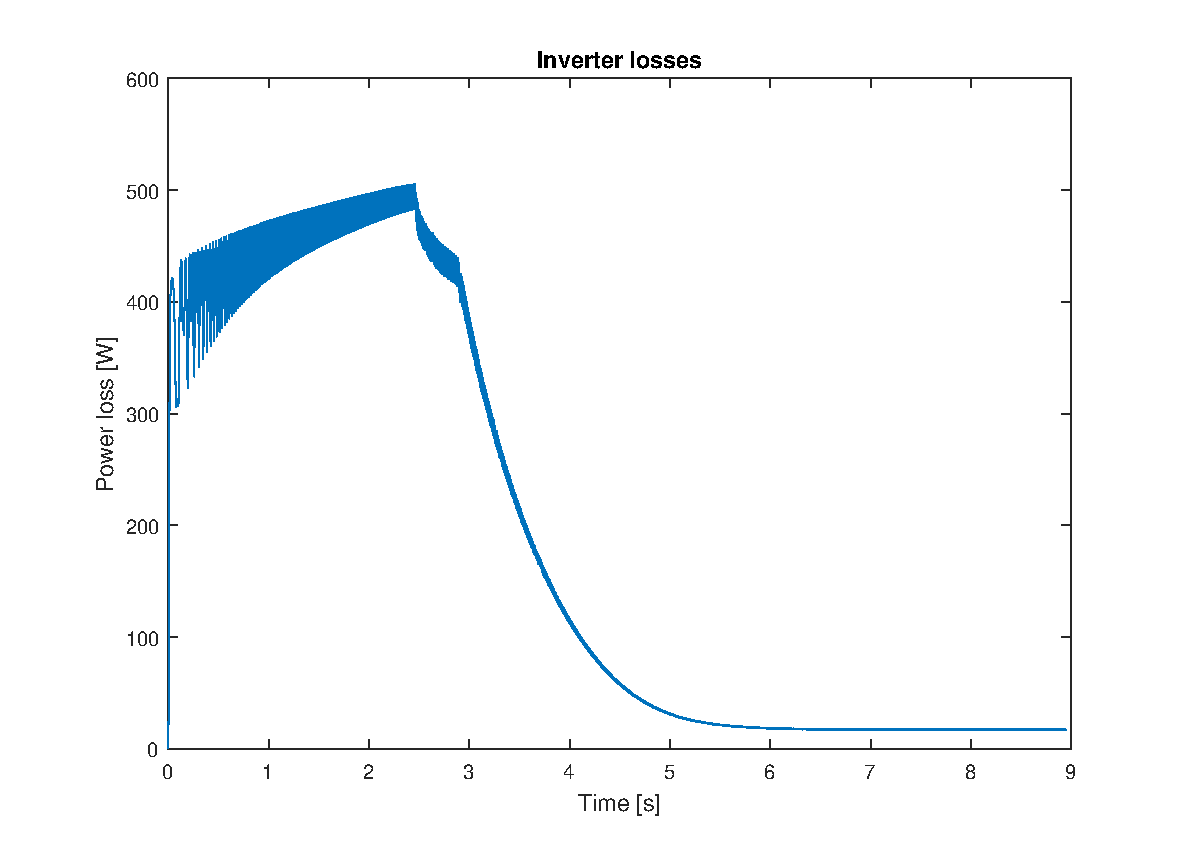
\includegraphics[width = \linewidth]{graphics/plecs_power_loss}
		\caption{Power loss in the MOSFETs}
		\label{fig:plecs_power_loss}
	\end{subfigure}
	\begin{subfigure}[t]{.49\linewidth}
		\centering
		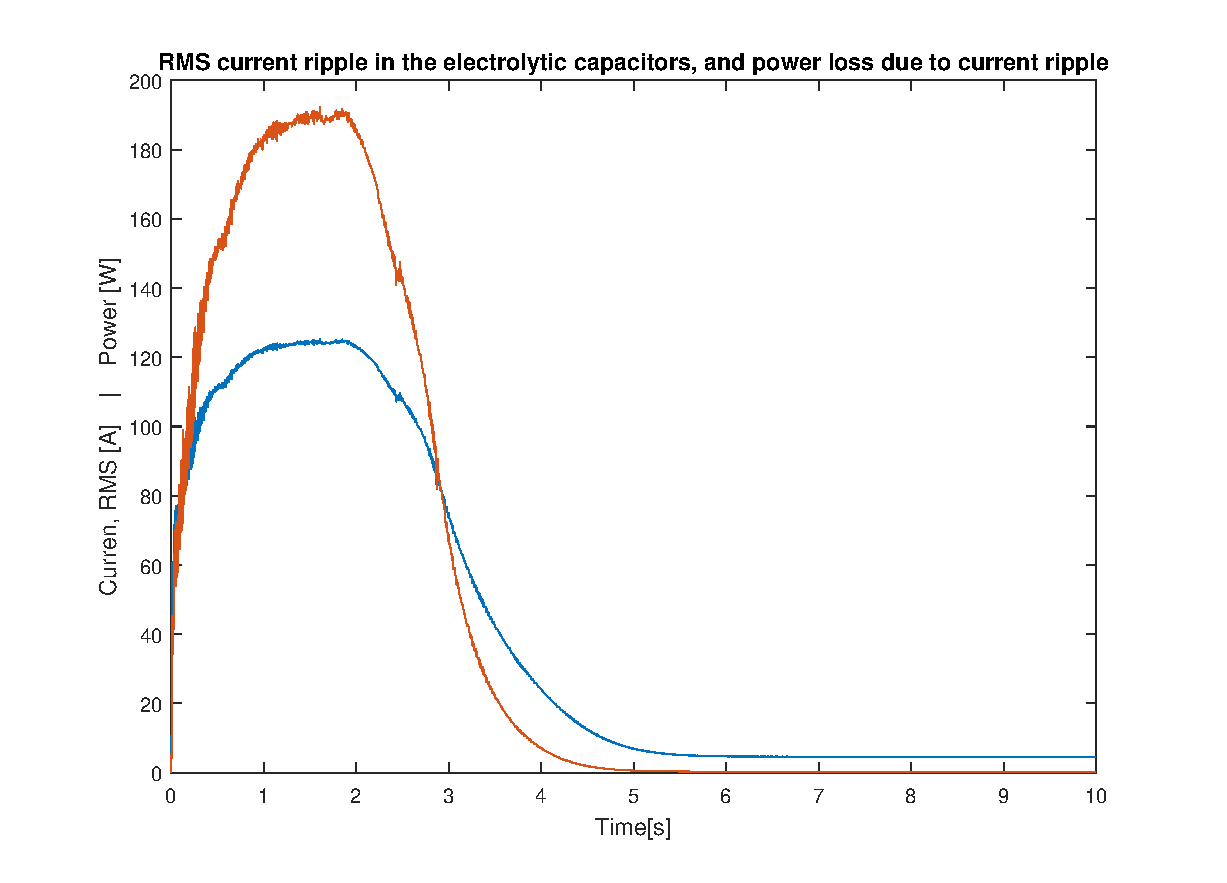
\includegraphics[width = \linewidth]{graphics/plecs_current_ripple}
		\caption{Current ripple in the electrolytic capacitors, in RMS.}
		\label{fig:plecs_current_ripple}
	\end{subfigure}
	\caption{MOSFET and capacitor loss.}
\end{figure}

The loss reaches a maximum of 500 \si{\watt}, which is lower than anticipated.
This might be because, the Plecs simulation takes into account for switchings that are not worst case scenario. 
Figure~\ref{fig:plecs_inverter_efficiency} displays the efficiency of the inverter. 

%\begin{figure}[H]
%	\centering
%	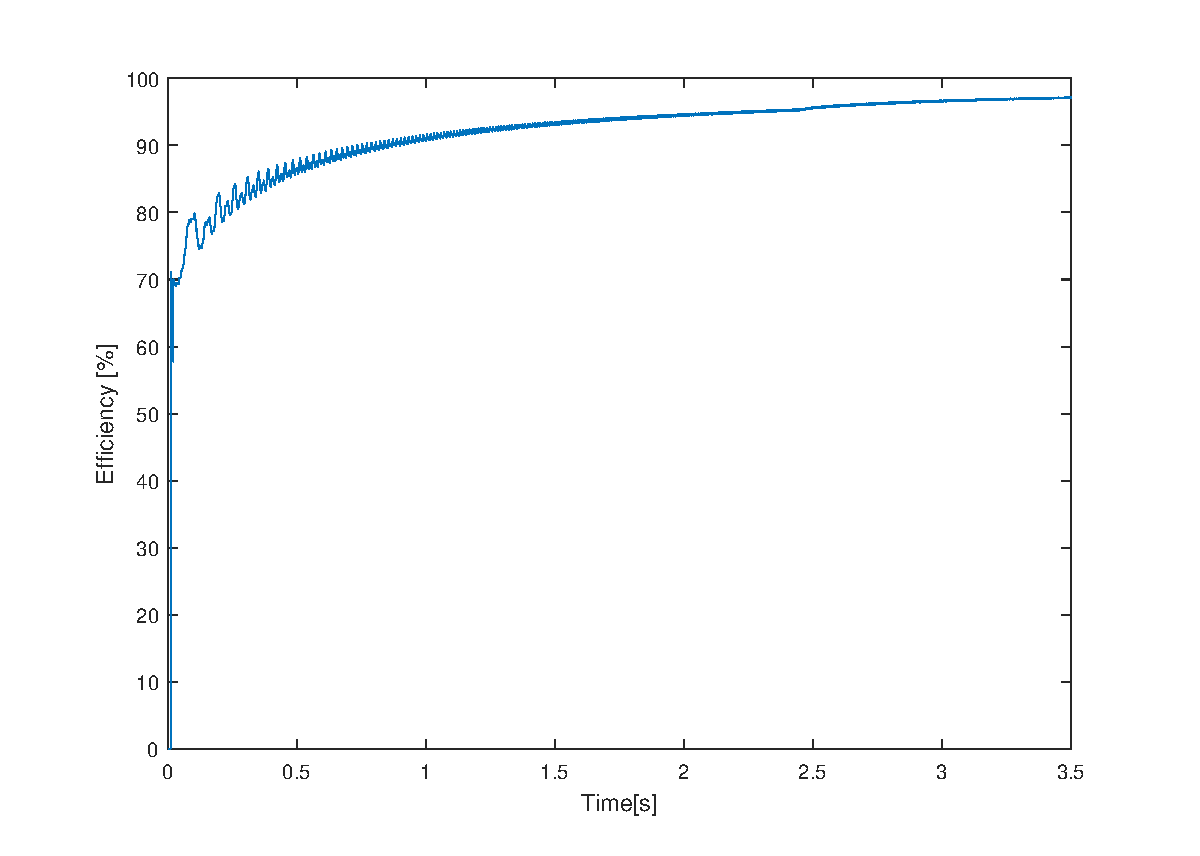
\includegraphics[width = 0.7\linewidth]{graphics/plecs_inverter_efficiency}
%	\caption{Efficiency of the inverter calculated from the electrical power going into the motor and the power lost in the MOSFETs}
%	\label{fig:plecs_inverter_efficiency}
%\end{figure}
The current ripple is displayed on figure~\ref{fig:plecs_current_ripple}

The large current ripple would result in up to 190 \si{\watt} of loss, which is a lot more than the capacitors can handle.
Not only is this power loss damaging for the efficiency of the inverter, it also produces a lot of heat, that is not absorbed by the heatsink.
A reason for this high number is likely the ideal switching used in Plecs. 
Because of this, the current from the supply can step from zero to 300 A instantaneously. 
In a more realistic simulation, stray inductances would limit the current slew rate. \\
Figure~\ref{fig:plecs_voltage_ripple} displays the voltage ripple of the capacitor bus.

\begin{figure}[H]
	\begin{subfigure}[t]{.49\linewidth}
		\centering
		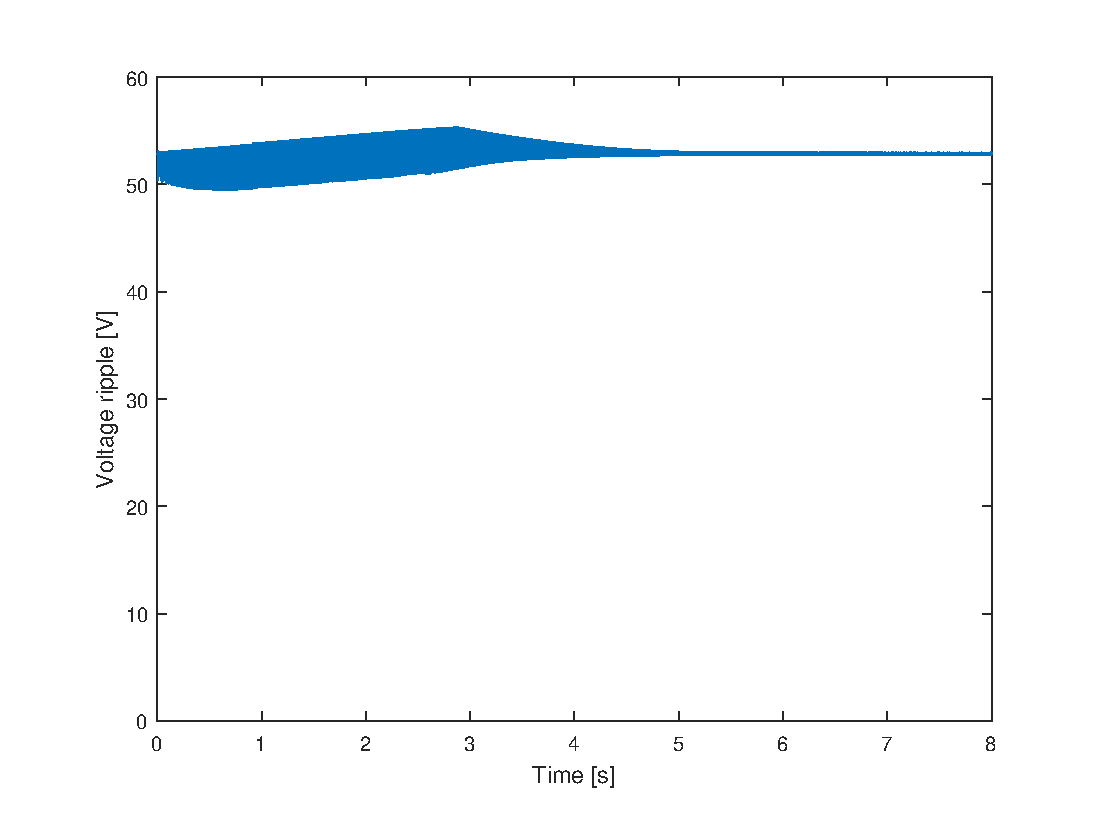
\includegraphics[width = \linewidth]{graphics/plecs_voltage_ripple}
		\caption{Voltage ripple on the inverter supply.}
		\label{fig:plecs_voltage_ripple}
	\end{subfigure}
	\begin{subfigure}[t]{.49\linewidth}
		\centering
		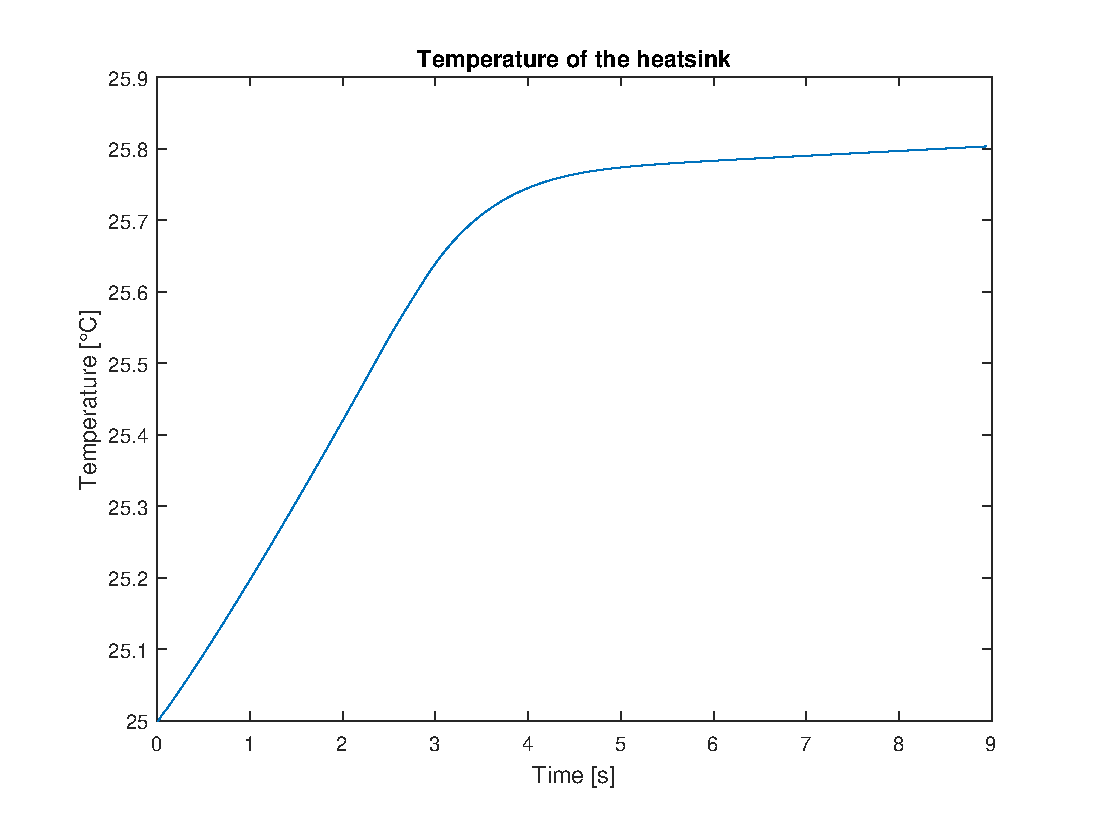
\includegraphics[width = \linewidth]{graphics/plecs_heatsink_temperature}
		\caption{Temperature increase of the heatsink.}
		\label{fig:plecs_heatsink_temperature}
	\end{subfigure}
	\caption{Voltage ripple and temperature profile.}
\end{figure}

The voltage ripple is quite low, less than 5 V, which means the inverter is supplied with an almost constant voltage, and the AC output is not begin disrupted by much.\\
Figure~\ref{fig:plecs_heatsink_temperature} displays the heatsink temperature  during the full throttle test

The temperature only increases 0.8 \si{\degree \celsius} during the test, so it easily handles the 500 \si{\watt} of heat generated by the MOSFETs. 
The reason for this limited temperature increase is the size of the thermal capacitance, rather than the low thermal resistance.\\

\subsubsection{Conclusion of Plecs simulations}\label{sub:plec_conclusion} 
It is possible to drive a PMAC motor with three phases of naturally sampled PWM. 
The inverter has a large thermal capacity, meaning that it would keep cool for the duration, it is being used. 
However, according to Plecs, the current ripple in the electrolytic capacitors greatly exceeds what they are rated for.
It was tried to add a ESL inductor to the capacitors, but that caused the simulation to become much slower to the point where it would not run at all.

\subsection{Simulation of the Over-Current Protection Circuit}
\label{sec:electricsimulation}
In order to verify the functionality of the OCP circuit discussed in section \ref{sec:ocpcircuit}, simulations of the circuit were conducted in LTSpice\footnote{LTSpice: Free simulation software by Linear Technologies.}.
The results of the simulation will be discussed in the order of the circuit.
As mentioned, only two of the phases are measured and the third will have to be calculated. 
This is done using the summing amplifier circuit shown in section \ref{sec:ocpcircuit}, repeated in figure \ref{fig:sumsimamp} for convenience.
The resulting signals can be seen on figure \ref{fig:sumsimresults}.
Clearly, P3 is not phase shifted 120\si{\degree} with respect to P1 or P2.
This is a consequence of using the non-inverting summing amplifier.

\begin{figure}[!h]
	\begin{subfigure}[b]{0.4\linewidth}
		\centering
		\includegraphics[width=\linewidth,trim=10cm 7.5cm 10cm 8cm]{graphics/sumamp}
		\caption{}
		\label{fig:sumsimamp}
	\end{subfigure}
	\begin{subfigure}[b]{0.6\linewidth}
		\centering
		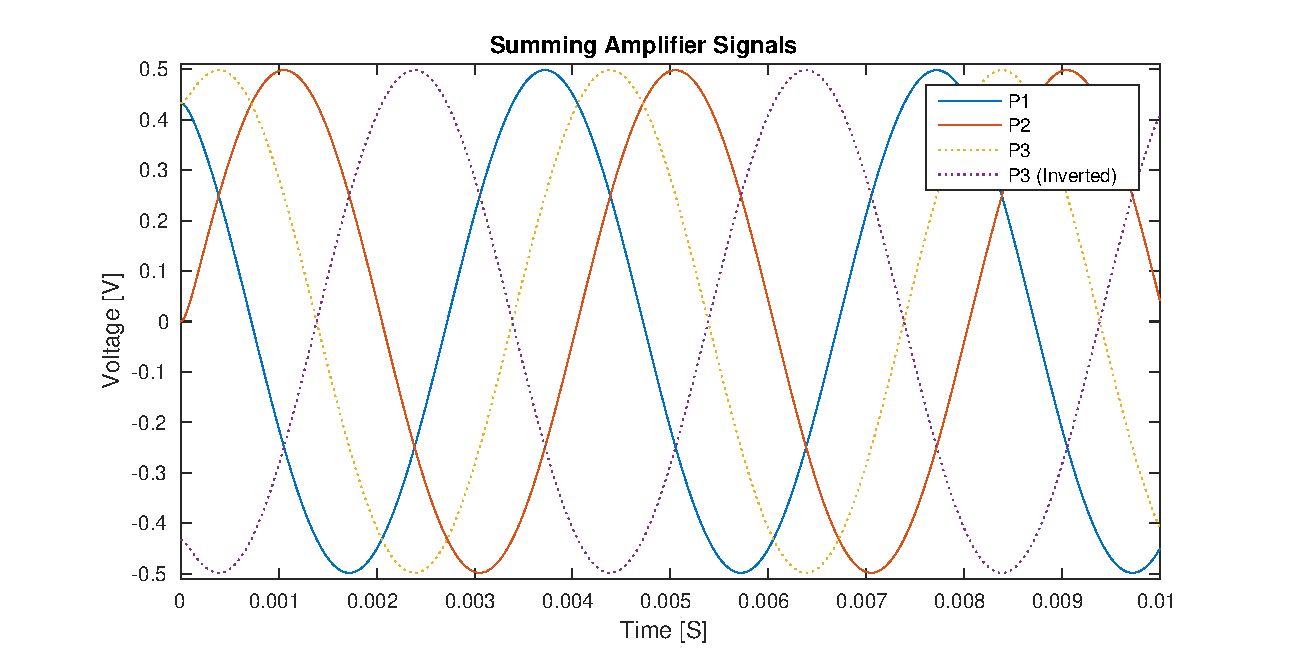
\includegraphics[width=\linewidth]{graphics/sumulation}
		\caption{}	
		\label{fig:sumsimresults}
	\end{subfigure}
	\caption{In \ref{fig:sumsimamp} is shown the summing amplifier used. In \ref{fig:sumsimresults} P1 and P2 represent the two measured phases while P3 is the calculated, third phase.}
	\label{fig:sumsim}
\end{figure}

Inverting P3 however, reveals the correct signal.
As all three signals, P1, P2 and P3 are rectified in the next step, this discrepancy is irrelevant.
For the remainder of this section only one phase is discussed as the circuitry of all three phases is identical after the initial summation.\\

The next step in the OCP process is the rectification of the signals.
This is done using a precision full wave rectifier as shown in figure \ref{fig:fullwaverectifier}.
As can be seen, the rectification error is relatively minor compared to the signal size.
It is mostly caused by the phase shifting done by the rectifier circuit.
This is apparent when noticing that the error is mostly identical between the rectified and non-rectified parts of the signal.

\begin{figure}[!h]
	\centering
	\includegraphics[width=.75\linewidth, trim=0cm 2cm 0cm 2cm]{graphics/fullwaverectifier}
	\label{fig:fullwaverectifier}
	\caption{Full wave rectifier used to rectify the current signals.}
\end{figure}

\begin{figure}[H]
	\begin{subfigure}[t]{.49\linewidth}
		\centering
		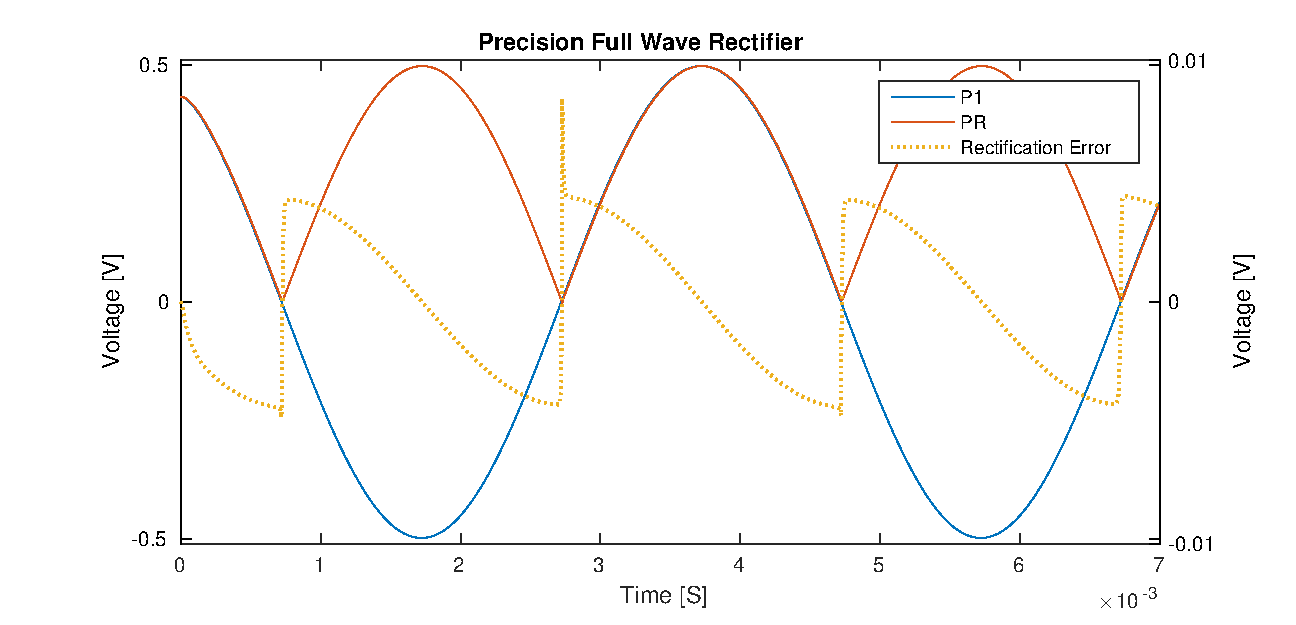
\includegraphics[width=\linewidth]{graphics/fullwaverectifiersim}
		\caption{}	
		\label{fig:fullwaverectifiersim}
	\end{subfigure}
	\begin{subfigure}[t]{.49\linewidth}
		\centering	
		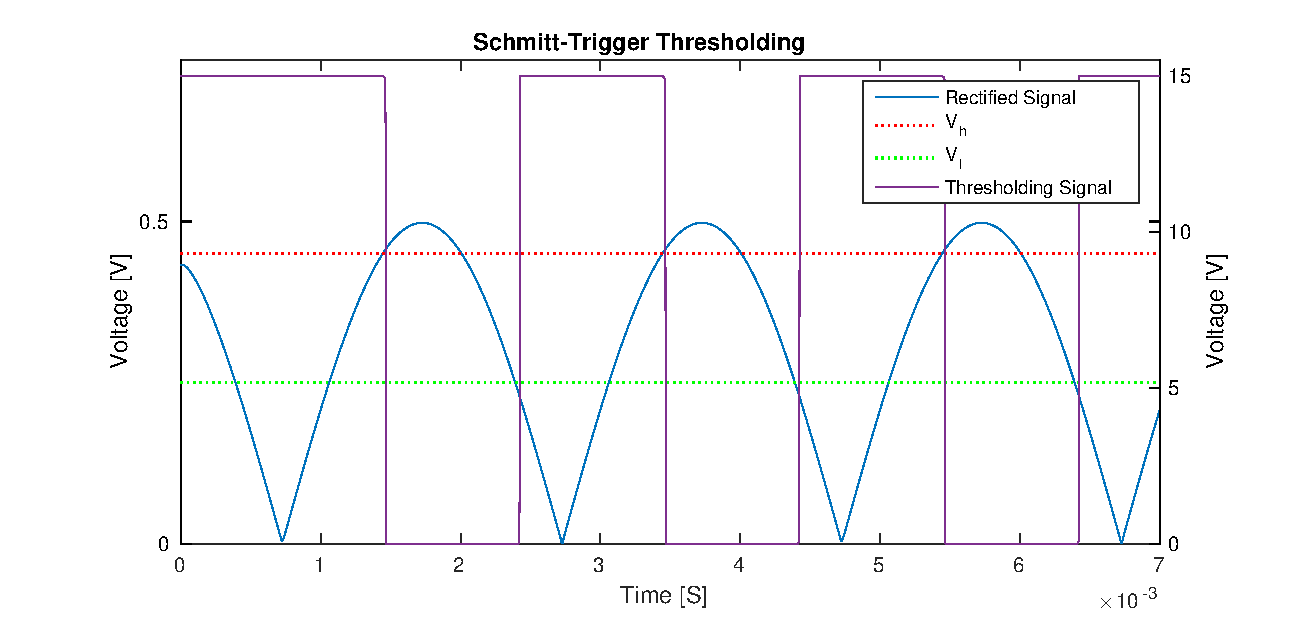
\includegraphics[width=\linewidth]{graphics/schmitt}
		\caption{}
		\label{fig:schmitt}
	\end{subfigure}
	\caption{\ref{fig:fullwaverectifiersim} shows the rectification error of the full wave rectifier. \ref{fig:schmitt} is an overview of the Schmitt triggered signal.}
\end{figure}

After rectification the signal is fed to a Schmitt-trigger with hysteresis voltages $V_h=0.475\si{\volt}$ and $V_l=0.25\si{\volt}$.
These signals are shown in figure \ref{fig:schmitt}.
The hysteresis values are reasonable close to the desired values, deviating only, by inspection, by a few \si{\milli\volt}.
This is expected since the resistor values calculated in section \ref{sec:schmitt} are rounded to the nearest standard value.
Additionally, in the real system there may be slight variations in components, these variations are not simulated however.\\

The remainder of the OCP circuit merely reverses the polarity of the signal.
This is done such that it conforms with the logical circuitry responsible for determining the state of the EN\_GATE signal discussed in section \ref{sec:electronics}.